Hexagon $ABCDEF$ is divided into four rhombuses, $\mathcal{P, Q, R, S,}$ and $\mathcal{T,}$ as shown.  Rhombuses $\mathcal{P, Q, R,}$ and $\mathcal{S}$ are congruent, and each has area $\sqrt{2006}$.  Let $K$ be the area of rhombus $\mathcal{T}$.  Given that $K$ is a positive integer, find the number of possible values for $K$.

\begin{center}
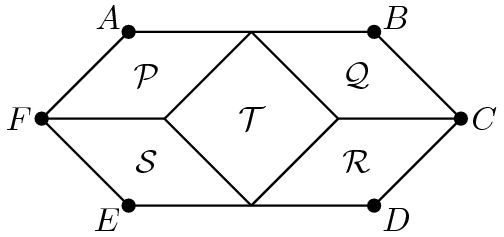
\includegraphics[width = 50.400000000000006mm]{img/fig0.png}
\end{center}